
\subsection*{3.9 Polygon Transformation}

Polygon transformation involves applying translation, rotation, reflection, enlargement, and shear to polygons while preserving or modifying their properties.

\textbf{Key Concepts:}
\begin{itemize}
	\item \textbf{Translation:} Moving every vertex of a polygon by a vector $\begin{pmatrix} a \\ b \end{pmatrix}$.
	\[
	\begin{pmatrix} x' \\ y' \end{pmatrix} =
	\begin{pmatrix} x + a \\ y + b \end{pmatrix}
	\]
	
	\item \textbf{Rotation:} Rotating a polygon by $90^\circ$ counterclockwise about the origin transforms each vertex:
	\[
	(x', y') = (-y, x).
	\]
	
	\item \textbf{Reflection:} Flipping a polygon across a given axis.
	\[
	\text{Reflection over the y-axis: } (x, y) \to (-x, y).
	\]
	\[
	\text{Reflection over the x-axis: } (x, y) \to (x, -y).
	\]
	
	\item \textbf{Enlargement:} Scaling a polygon by a factor $k$ about the origin:
	\[
	(x', y') = (kx, ky).
	\]
	
	\item \textbf{Shear:} Distorting a polygon along an axis while keeping one dimension fixed.
	\[
	\text{Horizontal shear: } (x', y') = (x + ky, y).
	\]
\end{itemize}

\textbf{Examples:}

\begin{flushleft}
	\textbf{Example 1: Translating a Triangle}
	
	A triangle with vertices $A(1,2)$, $B(3,4)$, and $C(5,1)$ is translated by the vector $\begin{pmatrix} -2 \\ 3 \end{pmatrix}$. Find the new coordinates.
	
	\textbf{Solution:}
	
	Using the translation formula:
	\[
	A'(1-2, 2+3) = (-1,5),
	\]
	\[
	B'(3-2, 4+3) = (1,7),
	\]
	\[
	C'(5-2, 1+3) = (3,4).
	\]
	
	\begin{center}
		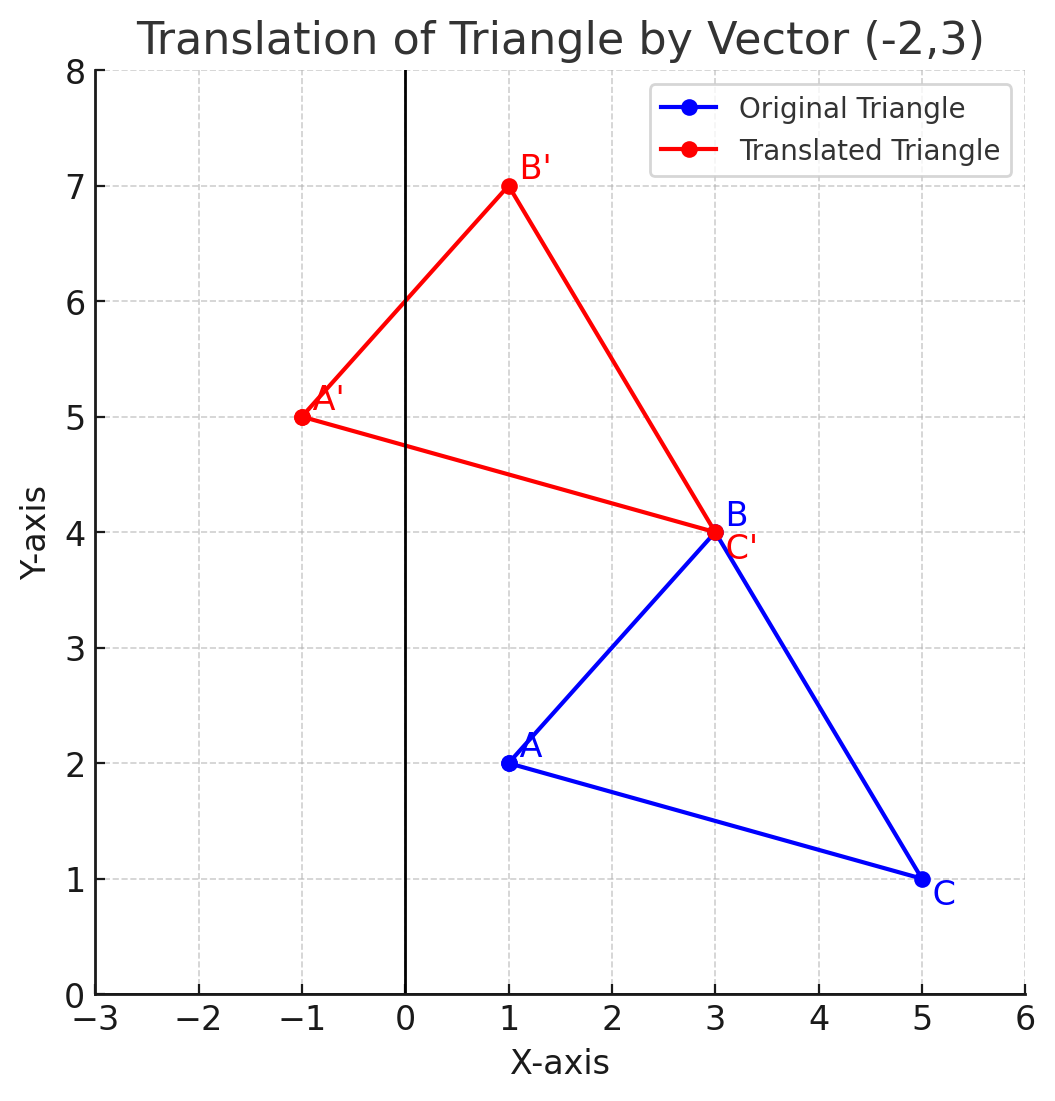
\includegraphics[width=0.6\textwidth]{3.17.png}
	\end{center}
	Thus, the translated triangle has vertices **$A'(-1,5)$, $B'(1,7)$, and $C'(3,4)$**.
\end{flushleft}

\begin{flushleft}
	\textbf{Example 2: Rotating a Square by $90^\circ$}
	
	A square has vertices $A(1,1)$, $B(3,1)$, $C(3,3)$, and $D(1,3)$. Find the new coordinates after rotating it $90^\circ$ counterclockwise about the origin.
	
	\textbf{Solution:}
	
	Using the rotation formula $(x', y') = (-y, x)$:
	\[
	A'(1,1) \to (-1,1),
	\]
	\[
	B'(3,1) \to (-1,3),
	\]
	\[
	C'(3,3) \to (-3,3),
	\]
	\[
	D'(1,3) \to (-3,1).
	\]
	\begin{center}
		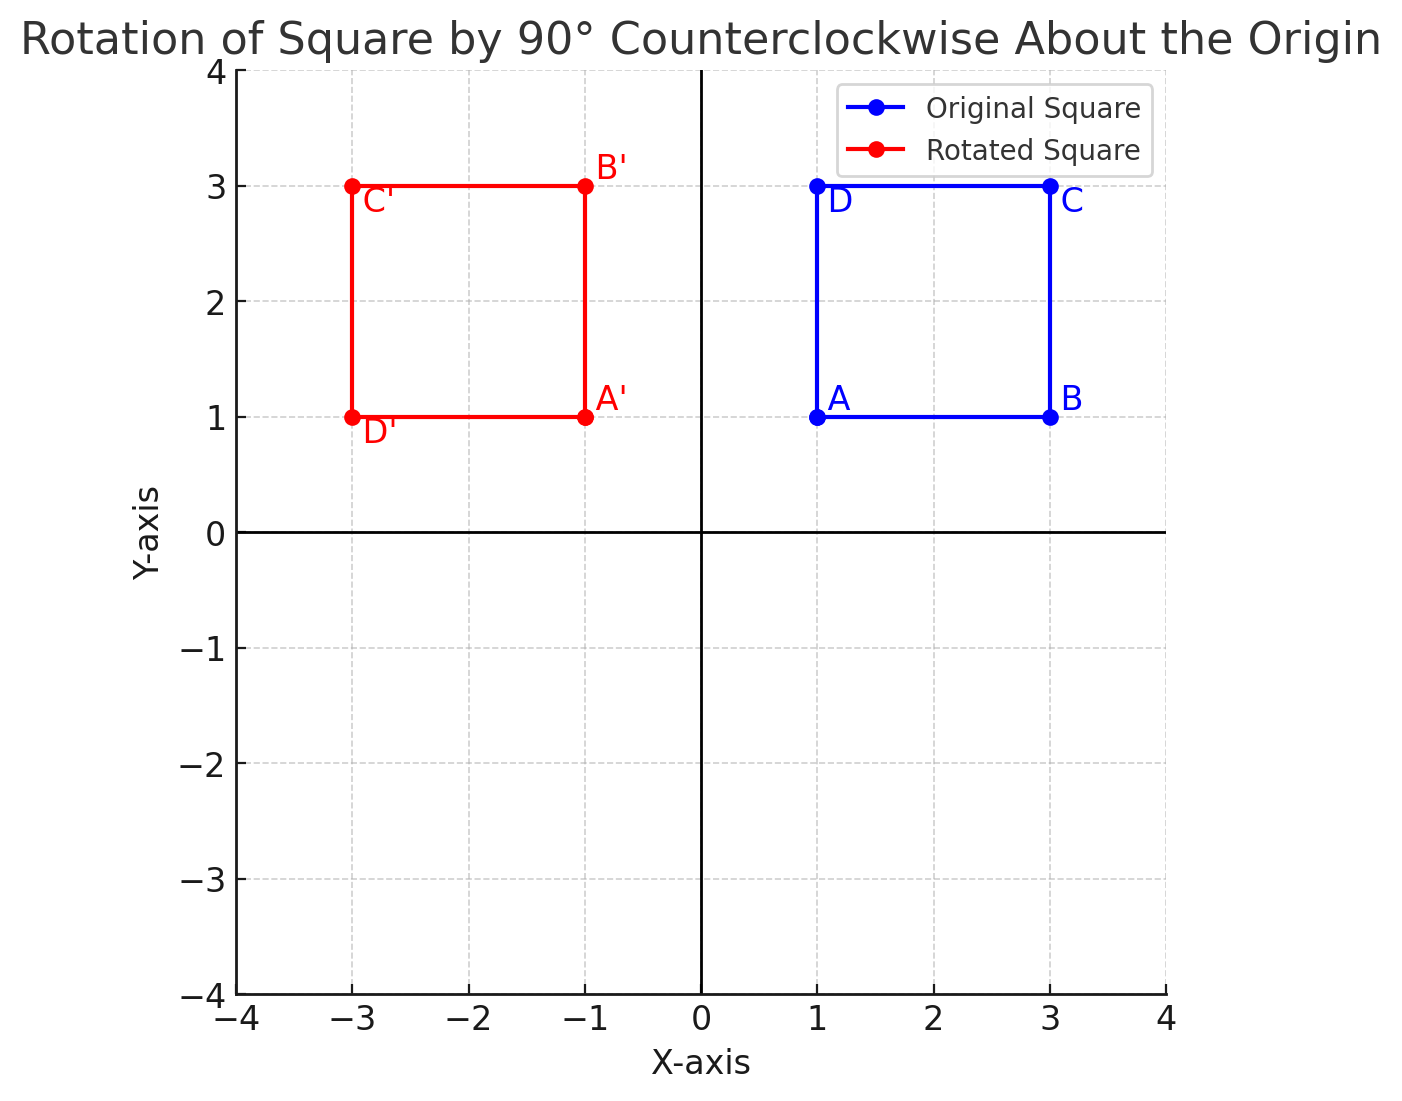
\includegraphics[width=0.6\textwidth]{3.18.png}
	\end{center}
	Thus, the rotated square has vertices **$A'(-1,1)$, $B'(-1,3)$, $C'(-3,3)$, and $D'(-3,1)$**.
\end{flushleft}

\begin{flushleft}
	\textbf{Example 3: Enlarging a Rectangle by Scale Factor 2}
	
	A rectangle has vertices $A(1,2)$, $B(4,2)$, $C(4,5)$, and $D(1,5)$. Find the new coordinates after enlarging it by a scale factor of 2 about the origin.
	
	\textbf{Solution:}
	
	Using the enlargement formula $(x', y') = (kx, ky)$:
	\[
	A'(1 \times 2, 2 \times 2) = (2,4),
	\]
	\[
	B'(4 \times 2, 2 \times 2) = (8,4),
	\]
	\[
	C'(4 \times 2, 5 \times 2) = (8,10),
	\]
	\[
	D'(1 \times 2, 5 \times 2) = (2,10).
	\]
	\begin{center}
		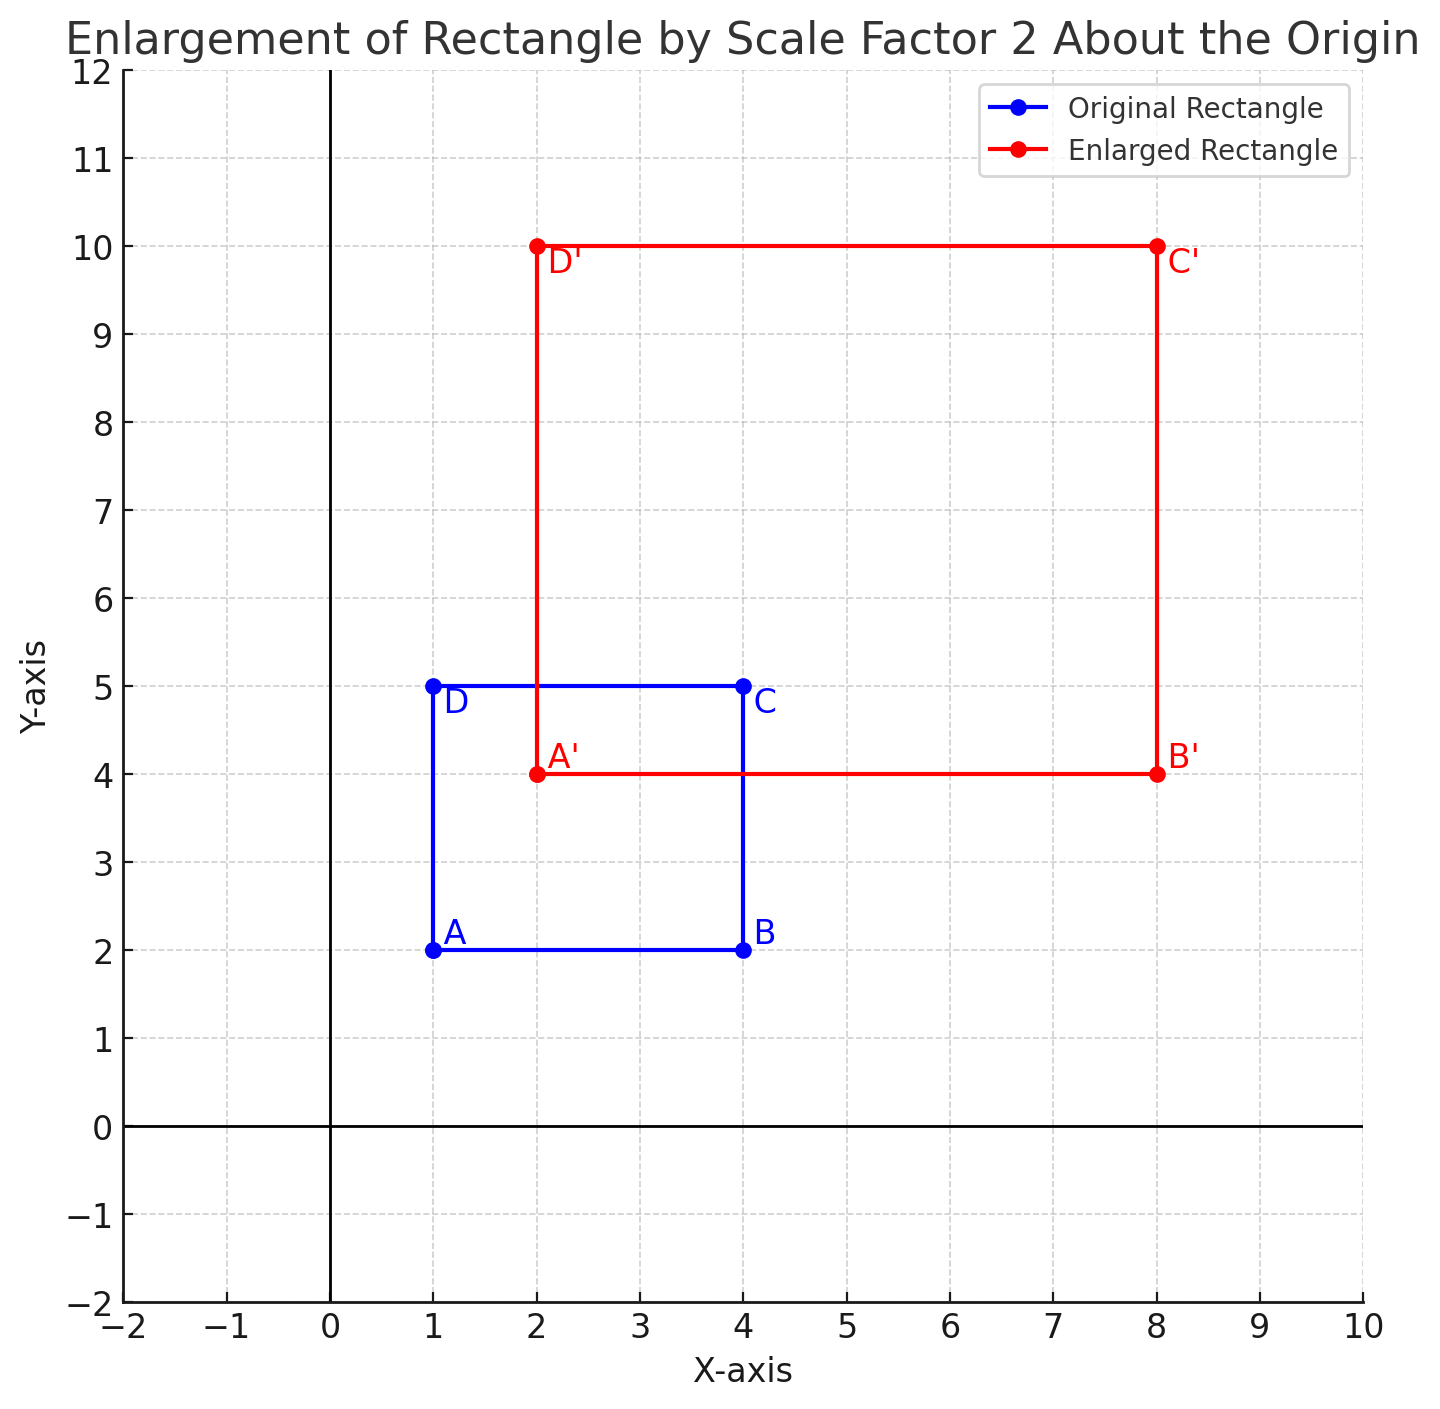
\includegraphics[width=0.6\textwidth]{3.19.png}
	\end{center}
	Thus, the enlarged rectangle has vertices **$A'(2,4)$, $B'(8,4)$, $C'(8,10)$, and $D'(2,10)$**.
\end{flushleft}

\begin{flushleft}
	\textbf{Example 4: Shearing a Parallelogram}
	
	A parallelogram has vertices $A(1,1)$, $B(4,1)$, $C(5,4)$, and $D(2,4)$. It is subjected to a horizontal shear transformation with shear factor $k=2$ along the $x$-axis. Find the new coordinates.
	
	\textbf{Solution:}
	
	Using the shear transformation formula:
	\[
	(x', y') = (x + ky, y).
	\]
	
	Applying the shear to each vertex:
	\[
	A'(1 + 2(1), 1) = (3,1),
	\]
	\[
	B'(4 + 2(1), 1) = (6,1),
	\]
	\[
	C'(5 + 2(4), 4) = (13,4),
	\]
	\[
	D'(2 + 2(4), 4) = (10,4).
	\]
	\begin{center}
		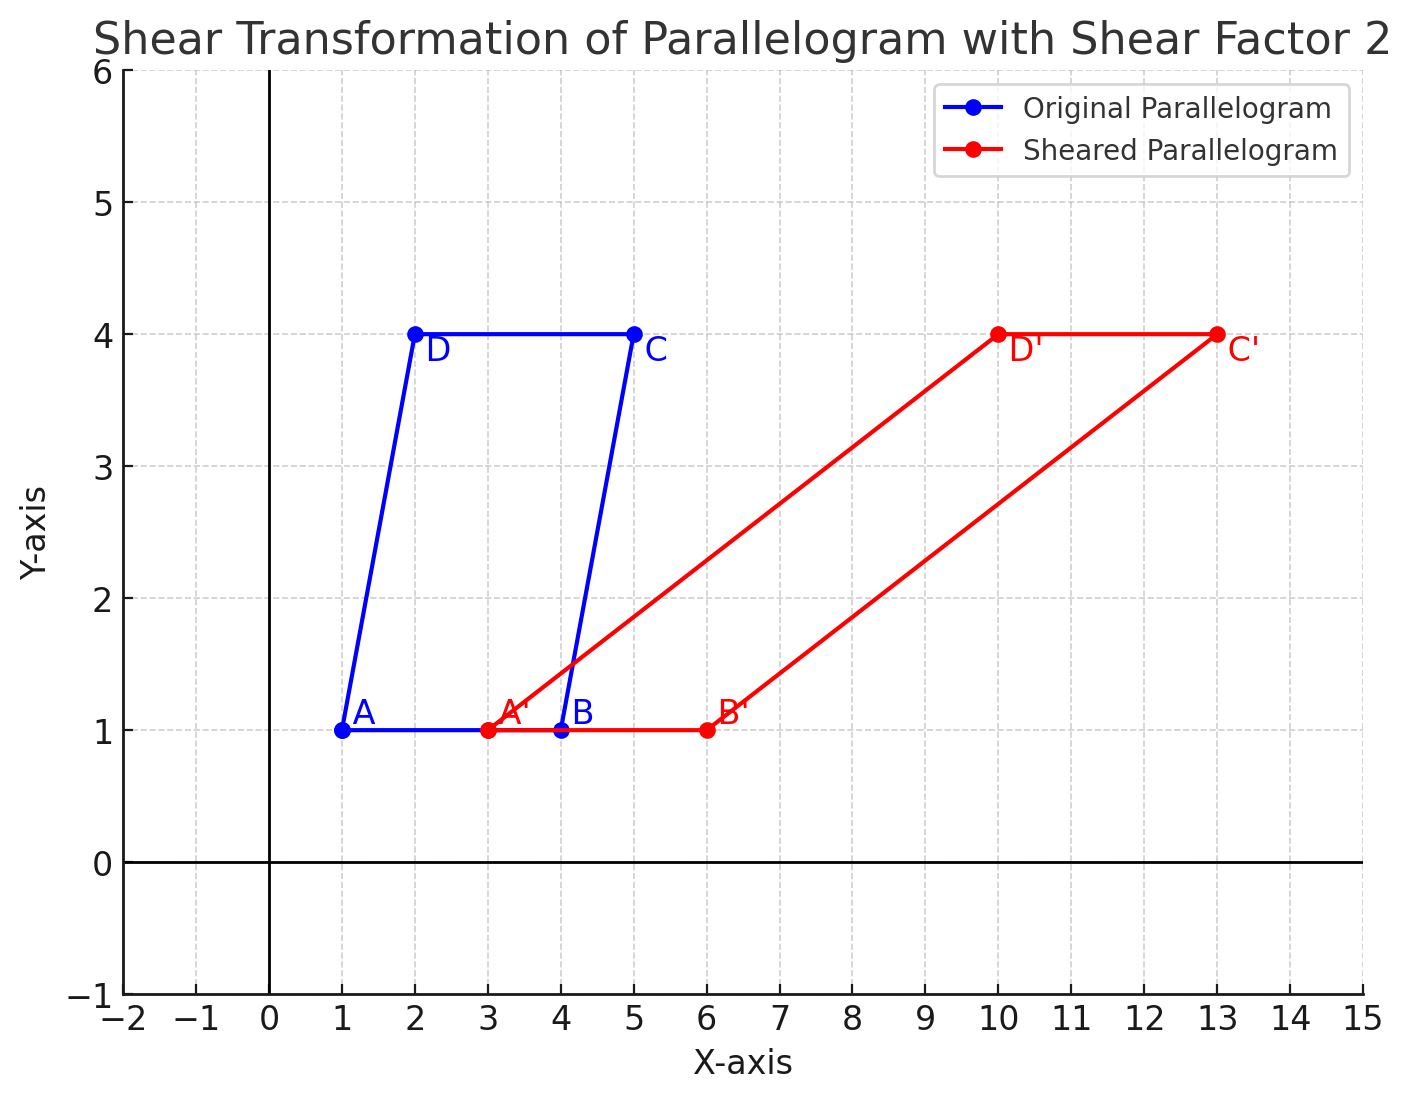
\includegraphics[width=0.6\textwidth]{3.20.png}
	\end{center}
	Thus, the sheared parallelogram has vertices **$A'(3,1)$, $B'(6,1)$, $C'(13,4)$, and $D'(10,4)$**.
\end{flushleft}
